\section{Method}
\subsection{Preparations}

The preparations consisted mainly of choosing which sensor to choose for the detection of the ball and how to mount it to the balance beam. After a series of test with both an ultrasonic sensor and an infrared sensor, the group came to a conclusion of using the latter. Using the built in plotter of the Arduino IDE and comparing the noise and accuracy of the two sensors. The result was that the IR-sensor was more consistent and linear than the ultrasonic sensor, thus easier to regulate.

After concluding towards the IR-sensor, the group decided to create several balance beam walls with different mounting heights, at a vertical position. Therefore the group could do further test to see what height the IR-sensor was the most effective and consistent at a stable position. 

In a vertical position, the IR-sensor was not perfectly lined up with the center of the ball, due to the the size of the sensor. This lead to misreading across the span of the beam. The group concluded to again change the wall mount. By mounting the sensor horizontally, the sensor aligned with the middle of the ball and the scaling issue was resolved. 

The group also concluded to flip the servomotor. This placed the connection point between the pole and balance beam closer towards the rotation point, resulting in a greater possible angle span on the balance beam. After connecting a 5V voltage regulator to the servo motor and a capacitor to the IR sensor, the preparations was finished and the group could continue with the regulation of the system. 
\subsection{Circuit}
The circuit was wired using mainly an arduino, breadboard, servo motor and a sharp distance sensor. In order to run the servo motor on the correct voltage we used a L7805, 5 volt voltage regulator. The capacitors are included to reduce electrical noise.

\begin{figure}[h]
    \centering
    \includegraphics[width = 1\textwidth]{Code/Images/Circuit-snip.png}
    \caption{Circuit design}
    \label{fig:Circuit design}
\end{figure}

\subsection{PID controller}

The group started the processes by looking at different examples and Arduino libraries for the PID controller. After reading through and testing multiple different Arduino PID libraries, the group decided to manually code the controller. The group used MATLAB to calculate and analyse different proportional, integral and derivative values using the given transfer function of the process.

\begin{equation}
    h(s) = \frac{r(s)}{\theta(s)}\ = \frac{mg\frac{d}{L}}{(\frac{J}{R^2}+m)s^2}
\end{equation}

Even though the IR-sensor had significantly less noise than the ultrasonic sensor, it was still enough to cause reading errors. Therefore the group decided to implement digital filters to the code. The implemented filters was a Kalman filter and a Median filter, both used to minimize noise in the sensor readings. 

However, as discussed in several classes, it is hard to make a perfect mathematical model of a practical problem. In the end the group concluded that trial and error for the parameter values was the plan going forwards. The parameters that needed to be adjusted were Kp, Ki, Kd, sample rate, Kalman filter, threshold and mapping of PID. After several hours of testing, discussion and plotting in MATLAB, the group used the following values for the mentioned parameters.\\

\begin{tabular}{r l}
   $K_p$ & 6\\
    $K_i$ & 0.15\\
    $K_d$ & 5000\\
    Sample rate & 25\\
Kalman filter \\
    Measurement uncertainty $KF_{mea}$ & 1.2 \\
    Estimation uncertainty $KF_{est}$ & 2 \\
    Process Variance $KF_{var}$ & 0.3 \\
Median filter\\
    Window size & 5 eller 3?\\
Threshold for the ball to settle & 0 $<$ threshold $<$ 1\\
Mapping of PID & (240, -240)\\
\end{tabular}

The group discovered that removing the integral constant from the PID massively reduced the settling time but proportionally increased the steady state error. Creating a threshold for the integral part of the PID to operate was an attempt to reduce the impact of the constant on the rest of the system, without removing it completely. 

As the ball entered the threshold some problems occurred. The IR-sensor still had minor noises even though the group implemented filters. Due to inconsistent sensor values, the settling time inside the threshold was slow. The group tried to solve this problem by adding a timer to the system. As the ball entered the set threshold, the PID was given a one second operating time before locking the output to the servo position This resulted in a fast settling time but a small inconsistent steady state inside that threshold.

The group aimed for the "excellent" requirements given in the task. The following goals were given:
\begin{center}
\begin{tabular}{ |c|c|c|c|}
 \hline
 Requirements & Excellent & Good & Fair \\
 \hline
 Stabilization time & $<$ 3 secs & $<$ 5 secs & $>$ 5 secs\\ 
 \hline
 Overshoot & $<$ 3 cm & $<$ 5 cm & $>$ 5 cm \\  
 \hline
 Oscillations in SS & None & $<$ +/- 5mm & $>$ +/- 5mm \\
 \hline
 Steady state error & $<$ 1 cm & $<$ 2 cm & $>$ 2 cm \\
 \hline
 Other & - & - & - \\
 \hline
\end{tabular}
\end{center}

In order to mitigate every factor we had to make a trade off. 

\subsection{MATLAB analysis}

The following code was used in MATLAB to analyse the system. The results were as expected and shows that we have chosen a configuration with a quick settling time and without overshoot.


\usemintedstyle{tango}
\inputminted[breaklines]{Matlab}{./Code/PID-Matlab.m}


\begin{figure}[h]
    \centering
    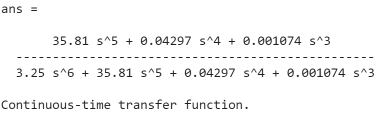
\includegraphics[width = 0.5\textwidth]{Code/Images/Tf.png}
    \caption{Matlab calculated transfer function}
    \label{fig:Matlab calculated transfer function}
\end{figure}

The calculated transfer function in figure \ref{fig:Matlab calculated transfer function} can be simplified to $\frac{35.81s^2+0.04297s+0.001074}{3.25s^3+35.81s^2+0.04297s+0.001074}$. This is the complete transfer function for our system.

\begin{figure}[h]
    \centering
    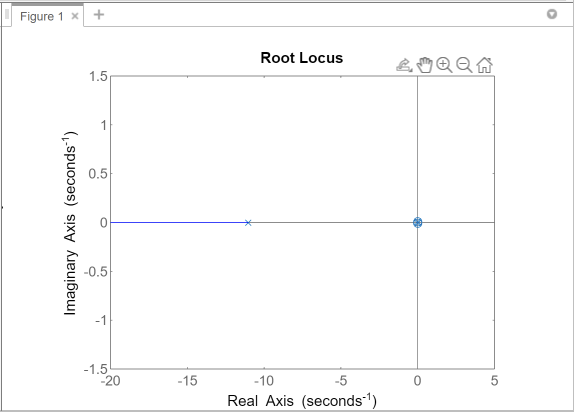
\includegraphics[width = 1\textwidth]{Code/Images/root-locus.png}
    \caption{Root locus plot}
    \label{fig:Root locus plot}
\end{figure}

The root locus shows a pole near 11. Two more poles and zeros are located near (0, 0.005) and (0, -0.005). They show when zoomed in.
The poles on the left hand side of the y-axis means that it is a stable system.

\begin{figure}[h]
    \centering
    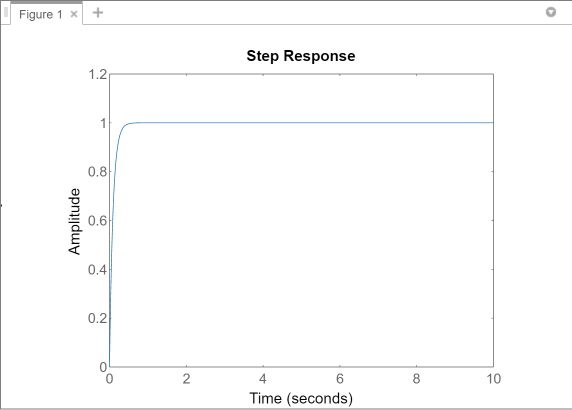
\includegraphics[width = 1\textwidth]{Code/Images/Step-Response.png}
    \caption{Step response}
    \label{fig:Step response}
\end{figure}

The step response of the system reveals a quick settling time and no overshoot.

